\section{Proof of concept: Monte Carlo simulation}

\begin{figure}[ht]
        \centering
        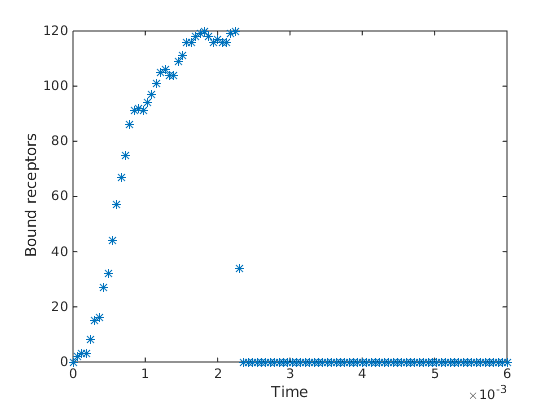
\includegraphics[width=0.45\textwidth]{boundReceptors}
        \caption{Number of bound receptors based on time.}
        \label{fig:boundReceptors}
\end{figure}

In order to make the problem simple enough to use a Monte Carlo simulation method, we postulate a few assumptions:
\begin{itemize}
\item We start with all 5000 neurotransmitters in one point, on the middle of the axon wall.
\item The probability of a neurotransmitter binding to a receptor is linearly dependent on how many receptors are available.
\item All neurotransmitters disconnect from the receptors when the signal is triggered.
\item Once the signal is triggered, glia cells are taken into account and start to clean up.
\item Neurotransmitters released from glia cells are marked as inactive and can again bond to the axon wall.
\item All probabilities of connecting a neurotransmitter to anything is dependent on the distance between the neurotransmitter and for example the dendritic wall.
\item We assume that the signal is triggered and passed on to the dendritic wall when we meet 80 percent coverage of the receptors.
\end{itemize}


As we can see in figure \ref{fig:boundReceptors}, the time before the synapse fires is around 2 ms. This is however higly dependent upon what constants we choose. An actual plot of what the simulation looks like is presented in figure \ref{fig:3dsim}. As for further studies, we deemed the simulation method not very easy to use (and extremely computationally expensive), so we instead turned to more traditional numerical mathematical modeling.


\begin{figure}[ht]
        \centering
        \begin{subfigure}[b]{0.45 \textwidth}
                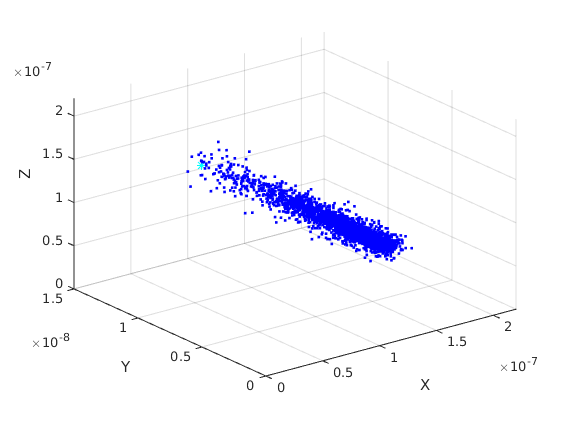
\includegraphics[width=\textwidth]{sim01}
                \caption{Some time has passed, a few neurotransmitters are bound to receptors.}
        \end{subfigure}
        ~
        \begin{subfigure}[b]{0.45 \textwidth}
                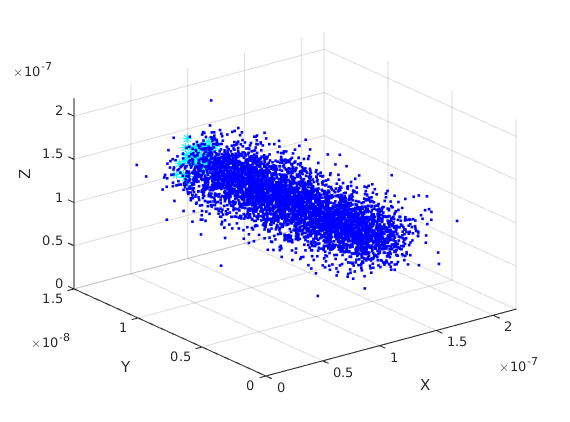
\includegraphics[width=\textwidth]{sim02}
                \caption{A large number of bounded neurotransmitters, dendrite almost ready to fire.}
        \end{subfigure}
        \\
        \begin{subfigure}[b]{0.45 \textwidth}
                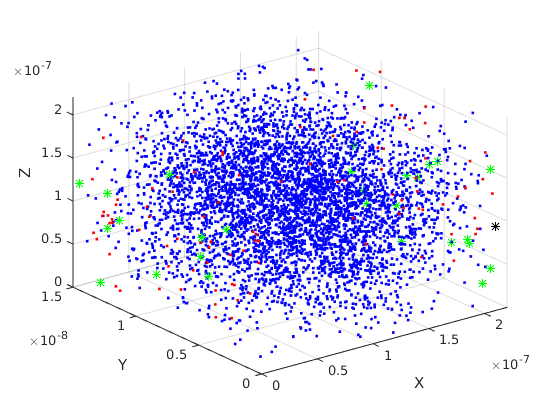
\includegraphics[width=\textwidth]{sim03}
                \caption{Dendrite has fired, glia cells have started to clean up the synaptic cleft.}
        \end{subfigure}
        ~
        \begin{subfigure}[b]{0.45 \textwidth}
                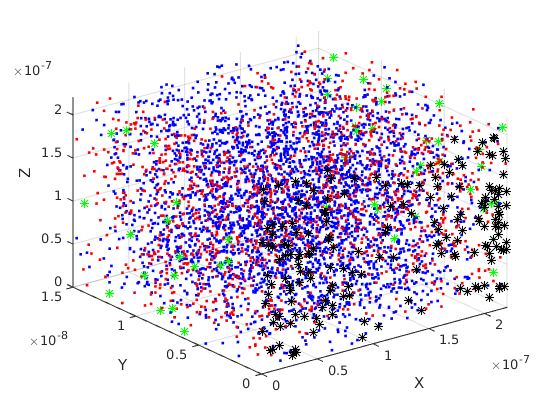
\includegraphics[width=\textwidth]{sim04}
                \caption{More time has passed, the first deactivated neurotransmitters has returned to the axon.}
        \end{subfigure}
        \caption{Monte Carlo simulation of the synaptic cleft. Active neurotransmitters are blue, inactive ones are red. Bounded neurotransmitters is indicated by a $*$ symbol and cyan is bound to receptors, green is bound to glia cells (transporters) and black ones have returned to the axon.}
        \label{fig:3dsim}
\end{figure}



